\documentclass{amsart}
\setlength{\textheight}{9in}
\setlength{\topmargin}{-0.25in}
\setlength{\textwidth}{7in}
\setlength{\evensidemargin}{-0.25in}
\setlength{\oddsidemargin}{-0.25in}
\usepackage{aaai}
\usepackage{amsfonts}
\usepackage[utf8]{inputenc}
\usepackage[T1]{fontenc}
\usepackage{graphicx} 
\usepackage[export]{adjustbox}
% needed to include these graphics
%\graphicspath{{./Pictures/}}      % only in case you want to keep the pictures in a separate
                                  % subdirectory; also see the appropriate line below
\usepackage{caption}
\usepackage{subcaption}
\usepackage{float}
\usepackage{framed}
\newcounter{temp}
\theoremstyle{definition}
\newtheorem{Thm}{Theorem}
\newtheorem{Prob}{Problem}
\newtheorem*{Def}{Definition}
\newtheorem*{Ans}{Answer}
\newcommand{\dis}{\displaystyle}
\newcommand{\dlim}{\dis\lim}
\newcommand{\dsum}{\dis\sum}
\newcommand{\dint}{\dis\int}
\newcommand{\ddint}{\dint\!\!\dint}
\newcommand{\dddint}{\dint\!\!\dint\!\!\dint}
\newcommand{\dt}{\text{d}t}
\newcommand{\dA}{\text{d}A}
\newcommand{\dV}{\text{d}V}
\newcommand{\dx}{\text{d}x}
\newcommand{\dy}{\text{d}y}
\newcommand{\dz}{\text{d}z}
\newcommand{\dw}{\text{d}w}
\newcommand{\du}{\text{d}u}
\newcommand{\dv}{\text{d}v}
\newcommand{\ds}{\text{d}s}
\newcommand{\dr}{\text{d}r}
\newcommand{\dth}{\text{d}\theta}
\newcommand{\bbR}{\mathbb{R}}
\newcommand{\bbN}{\mathbb{N}}
\newcommand{\bbQ}{\mathbb{Q}}
\newcommand{\bbZ}{\mathbb{Z}}
\newcommand{\bbC}{\mathbb{C}}
\newcommand{\dd}[2]{\dfrac{\text{d}#1}{\text{d}#2}}
\newcommand{\dydx}{\dfrac{\text{d}y}{\text{d}x}}
\renewcommand{\labelenumi}{{\normalfont \arabic{enumi}.}}
\renewcommand{\labelenumii}{{\normalfont \alph{enumii}.}}
\renewcommand{\labelenumiii}{{\normalfont \roman{enumiii}.}}
\font \bggbf cmbx18 scaled \magstep2
\font \bgbf cmbx10 scaled \magstep2
\usepackage{fancyhdr}
\usepackage{lipsum}
\usepackage{amsmath}
\usepackage{empheq}
\newcommand*\widefbox[1]{\fbox{\hspace{2em}#1\hspace{2em}}}
% Clear the header and footer
\fancyhead{}
\fancyfoot{}
% Set the right side of the footer to be the page number
\rfoot{\thepage}
\fancyhf{}
\pagestyle{fancy}
\begin{document}



%%%%%%%%%%%%%%%%%%%%%%%%%%%%%%%%%%%%%%%%%%%%%%%%%%%%%%%%%%%%%%%%%%%%%%%%%%%%%%%%%%%%%%%%%%%%%%%%%%%%%%%%%%%%%%%%%%%%%%%%%%%
%                                                                                                         Title Information
%%%%%%%%%%%%%%%%%%%%%%%%%%%%%%%%%%%%%%%%%%%%%%%%%%%%%%%%%%%%%%%%%%%%%%%%%%%%%%%%%%%%%%%%%%%%%%%%%%%%%%%%%%%%%%%%%%%%%%%%%%%
\LARGE{CIS 730: Artificial Intelligence}
 
\large
Project Report
 
John Boyington
\newline
\bigskip

%%%%%%%%%%%%%%%%%%%%%%%%%%%%%%%%%%%%%%%%%%%%%%%%%%%%%%%%%%%%%%%%%%%%%%%%%%%%%%%%%%%%%%%%%%%%%%%%%%%%%%%%%%%%%%%%%%%%%%%%%%%







%%%%%%%%%%%%%%%%%%%%%%%%%%%%%%%%%%%%%%%%%%%%%%%%%%%%%%%%%%%%%%%%%%%%%%%%%%%%%%%%%%%%%%%%%%%%%%%%%%%%%%%%%%%%%%%%%%%%%%%%%%%
%                                                                                            Objectives & Problem Statement
%%%%%%%%%%%%%%%%%%%%%%%%%%%%%%%%%%%%%%%%%%%%%%%%%%%%%%%%%%%%%%%%%%%%%%%%%%%%%%%%%%%%%%%%%%%%%%%%%%%%%%%%%%%%%%%%%%%%%%%%%%%

\section{Objectives \& Problem Statement}

%%%%%%%%%%%%%%%%%%%%%%%%%%%%%%%%%%%%%%%%%%%%%%%%%%%%%%%%%%%%%%%%%%%%%%%%%%%%%%%%%%%%%%%%%%%%%%%%%%%%%%%%%%%%%%%%%%%%%%%%%%%

StarCraft II is a popular competetive real-time strategy game.
To play successfully, players have to manage the game on both the micro-level with combat and structure placement and also at the macro-level making long-term strategic descisions.
The game is partially-observable, so exploration is required, several actions are available to the player at any given moment, things like movement and attacking happen in a continuous space and there are countless strategies used successfully.
For artificial intelligence, this game provides an excellent opportunity for research.
Recently, this game has been presented as a grand challenge in AI by DeepMind and Blizzard.

For the class project, the topic chosen was to develop a game-playing agent to master some component of this game.
More specificly, the plan was to develop a neural network to mimic the behavior of some scripted bot in the minigame `DefeatRoaches' in StarCraft II.
The hope is that through this research, more information might be gained on the process of learning through observing the action of others.
Large ammounts of replay data is available currently, including much from high-level players.
This data, in conjunction with these learned techniques may hold the key to teaching a machine to master the game.

Before starting the task there were a number of competencies I needed to develop before being able to actually the bot.
First, I would need to learn to use the StarCraft api that Blizzard and DeepMind had produced.
This python-based interface gives access to large ammounts of in-game information, like state variables and available actions, all provided in easy-to-use {\tt numpy} arrays.
This format is designed specifically with AI development in mind, and presents observation data and actions in ways that mimick human-like interpretation.

Learning Tensorflow was also necessary for the creation of the agent's neural network.
It's implementation allowed for the relatively simple creation and training of neural networks using keras.
Included in the appendix of this report is an example demonstrating the functionality of keras.

%%%%%%%%%%%%%%%%%%%%%%%%%%%%%%%%%%%%%%%%%%%%%%%%%%%%%%%%%%%%%%%%%%%%%%%%%%%%%%%%%%%%%%%%%%%%%%%%%%%%%%%%%%%%%%%%%%%%%%%%%%%






%%%%%%%%%%%%%%%%%%%%%%%%%%%%%%%%%%%%%%%%%%%%%%%%%%%%%%%%%%%%%%%%%%%%%%%%%%%%%%%%%%%%%%%%%%%%%%%%%%%%%%%%%%%%%%%%%%%%%%%%%%%
%                                                                                                 Background & Related Work
%%%%%%%%%%%%%%%%%%%%%%%%%%%%%%%%%%%%%%%%%%%%%%%%%%%%%%%%%%%%%%%%%%%%%%%%%%%%%%%%%%%%%%%%%%%%%%%%%%%%%%%%%%%%%%%%%%%%%%%%%%%

\section{Background \& Related Work}

%%%%%%%%%%%%%%%%%%%%%%%%%%%%%%%%%%%%%%%%%%%%%%%%%%%%%%%%%%%%%%%%%%%%%%%%%%%%%%%%%%%%%%%%%%%%%%%%%%%%%%%%%%%%%%%%%%%%%%%%%%%

It was in August 2017 that the paper introducing SC2LE (StarCraft II Learning Environment) was published and since then several papers have been published detailing methods used to approach the game \cite{vinyals2017starcraft}.
Within the paper itself was several baseline results published from the application of standard reinforcement learning (RL) algorithms.
Micro behaviors were considered by Liu et. al. who used a influence maps and potential fields to teach an agent various combat techniques \cite{liu2016evolving}.
Makar et. al. studied hierarchical multi-agent RL which broke down and decentralized learning tasks handled by separate agents \cite{makar2001hierarchical}.

Outside of AI, StarCraft II bot development has been happening for a long time now.
A paper by Onta\~n\`on et. al. compares the performance and architecture of the most competetive of these bots \cite{ontanon2013survey}.


%%%%%%%%%%%%%%%%%%%%%%%%%%%%%%%%%%%%%%%%%%%%%%%%%%%%%%%%%%%%%%%%%%%%%%%%%%%%%%%%%%%%%%%%%%%%%%%%%%%%%%%%%%%%%%%%%%%%%%%%%%%









%%%%%%%%%%%%%%%%%%%%%%%%%%%%%%%%%%%%%%%%%%%%%%%%%%%%%%%%%%%%%%%%%%%%%%%%%%%%%%%%%%%%%%%%%%%%%%%%%%%%%%%%%%%%%%%%%%%%%%%%%%%
%                                                                                                               Methodology
%%%%%%%%%%%%%%%%%%%%%%%%%%%%%%%%%%%%%%%%%%%%%%%%%%%%%%%%%%%%%%%%%%%%%%%%%%%%%%%%%%%%%%%%%%%%%%%%%%%%%%%%%%%%%%%%%%%%%%%%%%%

\section{Methodology}

%%%%%%%%%%%%%%%%%%%%%%%%%%%%%%%%%%%%%%%%%%%%%%%%%%%%%%%%%%%%%%%%%%%%%%%%%%%%%%%%%%%%%%%%%%%%%%%%%%%%%%%%%%%%%%%%%%%%%%%%%%%

The structure of the code will be considered within this section, as well as any techniques applied at various levels of implementation.
The highest level script it {\tt defeat\_roaches.py}.
It can be invoked with an command line arg, either {\tt learn} or {\tt log}.
This will select the whether you want the scripted bot, or the neural network to play the game.
Each agent is subclassed from a pysc2 built-in {\tt BaseAgent} class type and then the action used at each timestep is produced using the {\tt step} method of the agent.
At the highest level, you can choose things like the ammount of in-game steps before an action execution.
This can allow for an agent to be handicapped to play at the action-per-minute (APM) of a human player.
For this experiment, this parameter was set to 1, meaning that the agent acted after every frame.
It's at this level, too, that a {\tt Data\_Container} object is created and passed to agents.
This handles the access, logging, and handling of data produced by the scripted bot and used in the neural network.

For this particular problem, the observation data used was twofold.
Because of the nature of the training bot, access was needed to two different features from the observation.
The first, was the unit id to distinguish who owned which units.
The second was the unit health so the bot could target the unit with lowest health.
Before storage, however, this data was first put through a series of processing steps.
First, all values were scaled to between 0 and 1.
This is standard for neural net training and allows the network to more quickly fit functions to the data.
It was reasoned that, for an attack-only agent, the position of friendly units was irrelevent.
Therefore, all feature screen values associated with friendly units was set to zero, so only enemy units were visible.
Due to the ammount of data that was to be stored, image compression techniques were explored.
The intent was to reduce the ammount of space required to store the observation, while still maintaining the spatial features of the image.
It was found, via qualitative judgement, that compression from size 124x124 (the feature screen size) to 31x31 still allowed spatial features to be recognized within the image, but granted a reduction in size of a factor of 16.
An example of this image compression can be seen in the appendix.

The formulation of the action space was also considered.
Due to the continuous nature of the attack locations, the attack space was discretized so there were 30x25 potential locations, equally spaced apart.
These (x, y) pairs were flattened and then enumerated.
Each ``action id'' became a separate class the the network would attempt to train.

The {\tt data.py} file in the repo contains the {\tt Data\_Container} object.
This object accepts a {\tt timestep} as given by the api and then grabs the observation info needed.
It also accepts as an argument an {\tt action\_id} which logs the action taken by the scripted bot.
This data is then stored in a numpy array and saved to a file after each individual game is finished.

Two design philosophies governed the creation of the scripted agent.
The first is simplicity, as it will be easier to see if the learning bot is properly mimicking its actions.
The second is that it was designed in a way to exhibit unique and strategically useful micro behaviors.
The algorithm only takes one action, attacking, and always targets the enemy with lowest health.
Ties are broken with y-position.
This will focus down enemies that are the weakest to quickly remove them as a damage source.
The tiebreaker encourages the bot to flank the enemy units, a behavior that would be present and observable in the learning agent if correctly learned right.

After the scripted bot is used to generate data, the data is fed into the neural network.
This bot will process the data and try to memorize the actions associated with each observation with its neural network.
Because the network will output a class {\tt action\_id}, it simply needs retransformed into 2D (x, y) values and then the agent will attack that location.
The network has no hidden layers, just a length 1922 input and the 750 output nodes with relu activation.
The input dimention is a result of flattening the two 31x31 feature screens and the output dimension matches the number of potential actions available.

The game played was a minigame called `DefeatRoaches'.
The initial state of the game includes nine marines and four roaches, placed in random locations in a vertical formation on opposite sides of the screen.
The reward for defeating a roach is +10 and it's -1 for each marine defeated.
The end condition is 120 seconds or whenever all of the marines are defeated.
The fog of war in this minigame is relaxed and the camera is fixed, simplifying the tasks the agent needs to handle.

For the experiment, there was a total of 51433 traning data arrays.
The data was shuffled before being given to the network and then trained with a batch size of 64 and 3 epochs.
Both the training bot and learning bot were allowed to play 5 games each and the scores of each were recorded.

%%%%%%%%%%%%%%%%%%%%%%%%%%%%%%%%%%%%%%%%%%%%%%%%%%%%%%%%%%%%%%%%%%%%%%%%%%%%%%%%%%%%%%%%%%%%%%%%%%%%%%%%%%%%%%%%%%%%%%%%%%%








%%%%%%%%%%%%%%%%%%%%%%%%%%%%%%%%%%%%%%%%%%%%%%%%%%%%%%%%%%%%%%%%%%%%%%%%%%%%%%%%%%%%%%%%%%%%%%%%%%%%%%%%%%%%%%%%%%%%%%%%%%%
%                                                                                                                   Results
%%%%%%%%%%%%%%%%%%%%%%%%%%%%%%%%%%%%%%%%%%%%%%%%%%%%%%%%%%%%%%%%%%%%%%%%%%%%%%%%%%%%%%%%%%%%%%%%%%%%%%%%%%%%%%%%%%%%%%%%%%%

\section{Results}

%%%%%%%%%%%%%%%%%%%%%%%%%%%%%%%%%%%%%%%%%%%%%%%%%%%%%%%%%%%%%%%%%%%%%%%%%%%%%%%%%%%%%%%%%%%%%%%%%%%%%%%%%%%%%%%%%%%%%%%%%%%

% results table
\begin{table}[]
\caption{Comparison of the scores earned by both the scripted bot and the neural network in five games.}
\label{tab:scores}
\begin{tabular}{|l|l|l|}
\hline
Game & Scripted Bot & ANN  \\ \hline
1    & 126          & -8   \\ \hline
2    & 57           & 0    \\ \hline
3    & 117          & 2    \\ \hline
4    & 292          & 0    \\ \hline
5    & 210          & -8   \\ \hline
Avg. & 160.4        & -2.8 \\ \hline
\end{tabular}
\end{table}


Table \ref{tab:scores} shows the results from both of the bots.
The scripted bot demonstrated good performance, receiving an average score of 160.4 and a maximum score of 292.
For the learning bot, however, it had an average score of -2.8 and only a maximum score of 2.
The average accuracy for the learning bot was $1.2166 \times 10^{-3}$.
Qualitatively speaking, when the training accuracy was on the order of $1 \times 10^{-3}$, the agent would more confidently select an inaccurate point on the screen, cluster around that point and eliminate friendly units.
Another common behavior was becoming stuck looping back and forth through two points on either side of the friendly units.
When the accuracy was closer to $1 \times 10^{-3}$, the agents actions seemed entirely stochastic.


%%%%%%%%%%%%%%%%%%%%%%%%%%%%%%%%%%%%%%%%%%%%%%%%%%%%%%%%%%%%%%%%%%%%%%%%%%%%%%%%%%%%%%%%%%%%%%%%%%%%%%%%%%%%%%%%%%%%%%%%%%%






%%%%%%%%%%%%%%%%%%%%%%%%%%%%%%%%%%%%%%%%%%%%%%%%%%%%%%%%%%%%%%%%%%%%%%%%%%%%%%%%%%%%%%%%%%%%%%%%%%%%%%%%%%%%%%%%%%%%%%%%%%%
%                                                                                                                   Summary
%%%%%%%%%%%%%%%%%%%%%%%%%%%%%%%%%%%%%%%%%%%%%%%%%%%%%%%%%%%%%%%%%%%%%%%%%%%%%%%%%%%%%%%%%%%%%%%%%%%%%%%%%%%%%%%%%%%%%%%%%%%

\section{Summary}

%%%%%%%%%%%%%%%%%%%%%%%%%%%%%%%%%%%%%%%%%%%%%%%%%%%%%%%%%%%%%%%%%%%%%%%%%%%%%%%%%%%%%%%%%%%%%%%%%%%%%%%%%%%%%%%%%%%%%%%%%%%

Clearly, the learning agent was not successful in this endeavor.
There were a number of hinderences that caused this.
First, to classify that number of classes, the dataset was far too small.
The example in the appendix demonstrates successful classification of 10 classes using a dataset of 60,000 28x28 images, roughly the half the data used in this project.
Not only, that, but there was a large number of actions that were never taken by the scripted agent and therefore no data at all to train those.
Also, the action space enumeration orthogonalized the actions, meaning that it sacrificed its 2d nature.
Even though two attack target squares may be right next to eachother, they need separate data to train.
Ideally, there would be some correlation between nearby attack targets that would allow for easier training.

In future work, using attack policies may be better.
Specifically, scripted routines that would govern the different tactics that the agent could select between.
This would drastically reduce the number of classes needed to train.
Because this is an imitation exercise, the actions of the bot-to-be-imitated would need to be formulated in a way that matched the existing policies, but be different enough, that learning to imitate could still be a meaningful exercise.
There is also plenty of opportunity for RL techniques to be applied to this problem.

Ultimately, the problem of imitation here still remains largely unsolved.
Hopefully the application of some of these techniques described here will lead to partial solutions of this problem.

%%%%%%%%%%%%%%%%%%%%%%%%%%%%%%%%%%%%%%%%%%%%%%%%%%%%%%%%%%%%%%%%%%%%%%%%%%%%%%%%%%%%%%%%%%%%%%%%%%%%%%%%%%%%%%%%%%%%%%%%%%%







%%%%%%%%%%%%%%%%%%%%%%%%%%%%%%%%%%%%%%%%%%%%%%%%%%%%%%%%%%%%%%%%%%%%%%%%%%%%%%%%%%%%%%%%%%%%%%%%%%%%%%%%%%%%%%%%%%%%%%%%%%%
%                                                                                                                References
%%%%%%%%%%%%%%%%%%%%%%%%%%%%%%%%%%%%%%%%%%%%%%%%%%%%%%%%%%%%%%%%%%%%%%%%%%%%%%%%%%%%%%%%%%%%%%%%%%%%%%%%%%%%%%%%%%%%%%%%%%%


%%%%%%%%%%%%%%%%%%%%%%%%%%%%%%%%%%%%%%%%%%%%%%%%%%%%%%%%%%%%%%%%%%%%%%%%%%%%%%%%%%%%%%%%%%%%%%%%%%%%%%%%%%%%%%%%%%%%%%%%%%%


\bibliographystyle{aaai}
\bibliography{references}



%%%%%%%%%%%%%%%%%%%%%%%%%%%%%%%%%%%%%%%%%%%%%%%%%%%%%%%%%%%%%%%%%%%%%%%%%%%%%%%%%%%%%%%%%%%%%%%%%%%%%%%%%%%%%%%%%%%%%%%%%%%
%                                                                                                                  Appendix
%%%%%%%%%%%%%%%%%%%%%%%%%%%%%%%%%%%%%%%%%%%%%%%%%%%%%%%%%%%%%%%%%%%%%%%%%%%%%%%%%%%%%%%%%%%%%%%%%%%%%%%%%%%%%%%%%%%%%%%%%%%

\section{Appendix}

%%%%%%%%%%%%%%%%%%%%%%%%%%%%%%%%%%%%%%%%%%%%%%%%%%%%%%%%%%%%%%%%%%%%%%%%%%%%%%%%%%%%%%%%%%%%%%%%%%%%%%%%%%%%%%%%%%%%%%%%%%%

The Tensorflow website includes a basic classification example using the Fashion MNIST dataset.
It involves the creation of a neural network used to classify images based on which type of clothing it represents.
My example can be found in my project repository under {\tt agents/mnist/}.


\begin{figure}[h!]
    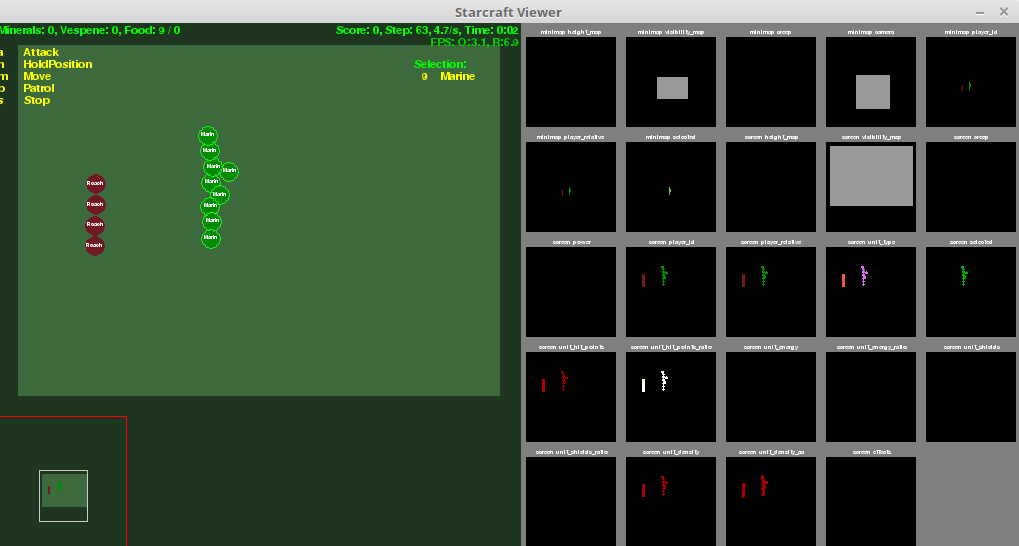
\includegraphics[width=1.0\linewidth]{gameplay}
    \caption{The pysc2 api visualized, showing the gameplay on the left and all of the feature screens on the right. Marines are represented by the green circles and the roaches by the red circles.}
\end{figure}


\begin{figure}[h!]
    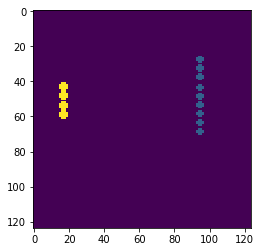
\includegraphics[width=1.0\linewidth]{fine}
    \caption{An image representing the {\tt player\_id} feature screen.}
\end{figure}

\begin{figure}[h!]
    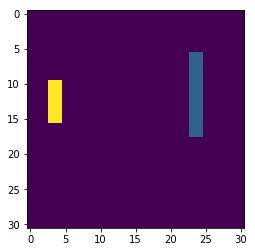
\includegraphics[width=1.0\linewidth]{course}
    \caption{An image representing the {\tt player\_id} feature screen, after have underwent the image compression techniques described above.}
\end{figure}

%%%%%%%%%%%%%%%%%%%%%%%%%%%%%%%%%%%%%%%%%%%%%%%%%%%%%%%%%%%%%%%%%%%%%%%%%%%%%%%%%%%%%%%%%%%%%%%%%%%%%%%%%%%%%%%%%%%%%%%%%%%










\end{document}
